\section{Approach and Technical Details}

% TODO: describe the elaboration pipeline
The general approach followed in this class project is based on the one adopted in \cite{Littlewort04dynamicsof,Bartlett06fullyautomatic}, where several concepts and algorithms are mixed and pipelined in order to achieve the not trivial task of the emotional states recognition. The methodology proposed on these papers is the following:

\begin{itemize}
\item Face detection and extraction
\item Facial features extraction via bank of Gabor filters.
\item Training several binary \emph{AdaBoost} classifiers with the labelled data (e.g.\ emotion labels).
\item Extraction of the most relevant features emerged after the training.
\item Most relevant facial features extraction based on valuable features observed.
\item Training several binary \emph{SVM} classifiers with the labelled data (e.g.\ emotion labels), using only most relevant features.
\end{itemize}

During project development we \emph{did not} rigidly follow the pipeline above for several pragmatical reasons, mainly related to the limited amount of time available for the class project. We adopted an approach based on a simplified version of this methodology. In detail our approach is based on the following steps:

\begin{itemize}
\item Face detection and extraction
\item Facial features extraction via bank of Gabor filters.
\item Training several binary \emph{Boost} classifiers with the labelled data (e.g.\ emotion labels).
\item Training several binary \emph{SVM} classifiers with the labelled data (e.g.\ emotion labels).
\end{itemize}

Further detail about reasons that have driven us to this approach can be found in~\ref{res:issues}.\\

In the following paragraphs we resume main characteristics of algorithms and datasets adopted in our class project.

% \cite{Littlewort04dynamicsof}
% \cite{Bartlett06fullyautomatic}
% \cite{learningOpenCV2008}

\subsection{Face Detection}

Face area represent the region of interest (ROI) in the context of this project, so we firstly focused on how to detect faces in an image. This kind of task has been widely discussed in literature and several algorithm implementation exists, in our case we choose to adopt a \code{Haar feature based cascade classifier}\cite{Viola01rapidobject}, which is also part of the OpenCV framework.\\
This detection methodology use an huge amount of simple Haar features to train an \emph{AdaBoost} cascade classifier. In detail the concept involved are:

\begin{description}
\item[Haar Features] this kind of features are calculated in a small windows of the image, in this window a binary mask is virtually applied and the value of the feature is the difference between the sum of the pixel values above the part of the mask with value 1 and the sum of the other part. An example of this kind of feature in fig.\ref{fig:haar}.
\item[Boosting] is a supervised machine learning approach that uses an ensemble of weighted \code{weak classifiers}. Further details in~\ref{appr:boosting}.
\item[Cascade Classification] this classification approach is based on several classification step, in each step a different feature is considered and if a feature value doesn't match the trained model the process is aborted and further stages are not evaluated.
\end{description}

\begin{figure}[!h]
\centering
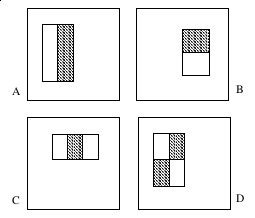
\includegraphics[width=4cm]{images/haarfeatures.png}
\label{fig:haar}
\caption{Haar feature example from \cite{Viola01rapidobject} }
\end{figure}

The OpenCV implementation also support \emph{multiscale detection}, which performs several detection steps rescaling the input image in order to identify object with different size with respect to the training sample sizes. High performance are reached thanks to the adoption of the \emph{integral image} for feature calculation. With this technique, a single haar-feature can be calculated with 3/4 lookups and a couple of arithmetic operations. The integral image is calculated with the following formula: $ ii(x,y) = \sum_{x' \leq x, y' \leq y}{ i(x',y') } $.\\

However, AdaBoost and Haar features are not the only choice, OpenCV implementation also support \emph{local binary patterns} based features and other boosting algorithms (eg. \code{RealBoost}, \code{GentleBoost}, \code{Discrete AdaBoost}, \ldots).

% \cite{Viola01rapidobject}

\subsubsection*{Face Rotation}

Our projects also implement a simple face rotation correction algorithm, which is based on the position of eyes detected via specifically trained cascade classifiers. Once eyes position is obtained a simple trigonometry calculation is performed in order to get the value of the angle between the eye-line and the x-axis, this value is then used for the definition of rotation matrix which is applied to the whole image.

\subsection{Gabor Filters}

Roughly speaking Gabor filters are \emph{linear} filter obtained by modulating a complex sinusoid with a \emph{Gaussian}, this kind of filters is typically used in image processing for tasks like edge detection, texture classification and face recognition\cite{gaborApplication}. These filters result particularly effective in case of a time-frequency analysis, which is an analysis technique that aims to study a signal in both time and frequency domain \emph{simultaneously}, due to multi-resolution\footnote{Multi-resolution is a method for orthonormal base creation by slicing the signal space into subspaces at different scales} and multi-orientation properties. One reason of the great success of this kind of filters is the discovery that simple cells in the human visual cortex can be modelled with this particular filter. In our project we adopt the following Gabor function formula:

\begin{equation}
g(x,y,\lambda,\theta,\psi,\sigma,\gamma) = \exp \left( - \frac{ x'^2 + \gamma^2 y'^2 }{ 2 \sigma^2} \right ) \exp \left( i \left( 2 \pi \frac{x'}{\lambda} + \psi \right ) \right )
\end{equation}

Where $x' = x \cos\theta + y \sin\theta$ and $y' = -x \sin\theta + y \cos\theta$ represent the rotated component of the complex sinusoid, $\lambda$ is the wavelength of the sinusoid, $\theta$ is the spatial orientation of the filter, $\phi$ is the phase offset, $\sigma$ is the standard deviation of the Gaussian support and $\gamma$ is the aspect ratio factor (eg. 1.0 for a circular shape).

Also derived parameters could be considered, for example the spatial frequency \emph{bandwitdh} of the filter is defined as:

\begin{equation}
b = log_2 \left ( \frac{ \frac{\sigma}{\lambda} \pi + \sqrt{ \frac{ln(2)}{2} )} }{  \frac{\sigma}{\lambda} \pi - \sqrt{ \frac{ln(2)}{2} )} } \right ),  \frac{\sigma}{\lambda} = \frac{1}{\pi} \sqrt{ \frac{ln(2)}{2} } \frac{2^b+1}{2^b-1} 
\end{equation}
These additional relationship between $\lambda$, $\theta$ and $b$ could be useful for generating Gabor filter banks\cite{gaborParams}. 

\subsubsection*{Gabor Filter Bank}
Gabor Filter banks are one of the main methodes for selection Gabor filters typically adopted in texture segmentation problems, families of filters are typically obtained by generating Gabor kernels with spatial frequencies $\lambda$, sinusoid orientation $\theta$ and bandwidth in ad hoc intervals while scaling parameters are sometimes selected intuitively and assumed to be constant. 

Our implementaion rely on a slightly modified version of the \code{OpenCV} Gabor kernel function, in detail we have added the capability to generate the imaginary part of the Gabor function too, wich is missing in the original implementation.

\subsubsection*{Gabor Energy Filters}
One of the basic way to deal with complex Gabor filter is to consider the magnitude of the filter response and considering the energy response of the filter. In our implementation we used the euclidean norm $ \left \| g \right \|_2 = \sqrt{ g_{real}^2 + g_{imag}^2 }$ due to the separate calculation of both imaginary and real part.

\begin{figure}[!h]
\centering
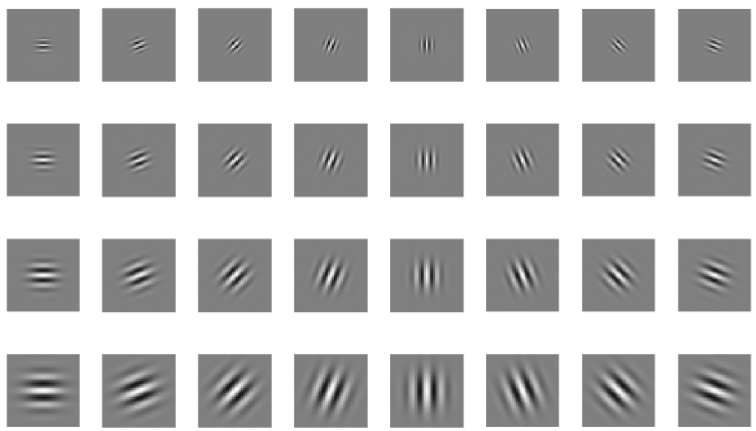
\includegraphics[width=12cm]{images/gabor.png}
\label{fig:gabor}
\caption{Gabor filter bank from \cite{gaborApplication} }
 \end{figure}


% \cite{gaborTutorial}
% \cite{gaborApplication}
% \cite{Lades93distortioninvariant}
\newpage
\subsection{Boosting}
\label{appr:boosting}

Boosting is a powerful learning concept that combines the performance of many ``weak'' classifiers to produce a ``strong'' one. For ``weak classifier'' is intended a generic classifier that performs slightly better than random choice, this non-restrictive requirement open new prospective for simple and computationally cheap classifiers (eg. simple thresholds). Boosting is a sort of meta-algorithm that can be applied in a numerous scenario adopting different weak classifiers, different weighting scheme, or also different error function. The general concept behind this supervised learning strategy is the weighting and re-weighting of the features in order \emph{focus on the mis-predictions}\cite{rojas2009adaboost}.

A classical case of boosting algorithm is the Adaptive Boost (\code{AdaBoost})\cite{Friedman98additivelogistic}, one of the first boosting approaches proposed. For this reason we briefly introduce its behaviour:

\begin{algorithm}
\caption{Discrete AdaBoost algorithm (binary classification)} 
\label{alg:adaboost}
\begin{algorithmic}
\STATE $i=1 \ldots T$ training data, $x_i$ is sample and $y_i \in \{-1,+1\}$ is label
\STATE $w_{i}^{(1)}=1$ is the initial weight of $x_i$
\STATE $N$ iteration number
\STATE $M$ classifier number
\STATE $W$ is the sum of weights of all data points
\STATE $W_e$ is sum of weight of data where considered classifier yields wrong label
\FOR{$i \in 1 \ldots N$ } 
%	\FOR{$m \in 1,\ldots,M$ } 
		\STATE find classifier $k_{m}(x)$ which minimize $W_e=\sum_{y_i \neq k_m(x_i)}{w_{i}^{(m)}}$
		\STATE set weight of classifier to $\alpha_{m}=\frac{1}{2}ln(\frac{1-e_m}{e_m}) $, where $e_m=W_e/W$
		\IF{$k_m(x_i) $ is a miss} 
	 		\STATE update weights $w_{i}^{(m+1)}=w_{i}^{(m)}e^{\alpha_m}=w_{i}^{(m)}\sqrt{\frac{1-e_m}{e_m}}$
		\ELSE
			\STATE update weights $w_{i}^{(m+1)}=w_{i}^{(m)}e^{-\alpha_m}=w_{i}^{(m)}\sqrt{\frac{e_m}{1-e_m}}$
 		\ENDIF
%\ENDFOR
\STATE output $sign( \sum_{m \in 1 \ldots M}{ \alpha_m k_m (x)} )$
\ENDFOR
\end{algorithmic}
\end{algorithm}

\code{OpenCV} framework implements several AdaBoost variants like \code{Real AdaBoost}, where weak classifiers may express class probabilities $p_m(x)$ instead of $\{-1,+1\}$ values, and \code{Gentle AdaBoost} which updates weight differently $\alpha_{m}=P(y_i=1|x_i)-P(y_i=0|x_i)$. 

% \cite{rojas2009adaboost}
% \cite{Friedman98additivelogistic}

\subsection{SVM}

Support Vector Machine (\emph{SVM}) is a machine learning approach that
 constructs an hyperplane, which maximizes the distance between the training
 data of any class, performing a classification.
 
 Since results in \cite{Littlewort04dynamicsof} show that linear SVM performs
 slightly better than non-linear approaches, we used only \emph{Linear SVM} for
 its faster training speed. Specifically, we used the linear SVM implementation
 of \emph{OpenCV}, which realizes a \emph{C-Support Linear SVM}, or \emph{Linear
 SVM} with \emph{Soft Margin}.
 
 \begin{align}
   \min & \frac{1}{2} \boldsymbol{\omega}^T \boldsymbol{\omega} + C*\sum_{i=1}^l \xi_i\\
   & y_i * (\boldsymbol{\omega}^T \phi(\textbf{x}_i) + b) \geq 1 - \xi_i,\\
   & \xi_i \geq 0, i = 1, \dots, l
   \label{mt:lin_svm}
 \end{align}
 
 Where $\boldsymbol{\omega} \cdot \textbf{x} - b = 0$ is the hyperplane:
 $\boldsymbol{\omega}$ is the normal vector to the hyperplane and $\textbf{x}_i
 \in \mathbb{R}^n, i = 1,\dots,l$ are the training vector.  $y \in \mathbb{R}^l,
 y_i \in \{1, -1\}$ is a class indicator, $\xi_i$ is a non-negative slack
 variable measuring the degree of misclassification on $\textbf{x}_i$. The
 parameter $C$ gives a weight to these misclassification variables. In other
 words, $C$ is a tradeoff between margin maximization and error minimization

\subsection{Dataset}

Access to properly labelled data is not a trivial aspect when dealing with supervised machine learning algorithm, especially when you are not trained to label that kind of data. Emotion labelling is not a task that someone can improvise: training manual like \emph{Facial Action Coding System (FACS) Manual} exists and certifications are required in order to prepare scientifically acceptable dataset.
 
For this reason we required access to the ``Cohn-Kanade Expression Database''\cite{Kanade2000} which contains 486 sequences from 97 posers, each sequence is tagged with FACS, contains facial feature tracking data and also have \emph{emotion labels}. This dataset is considered is a \emph{``must have''} from the academical community, in fact the great part of the publications about topic related to \emph{faces} cite it as one of the adopted dataset.

% \cite{Kanade2000}

